\documentclass[11pt,a4paper]{article}
\usepackage[margin=2.3cm]{geometry}
\usepackage{amsmath,amssymb}
\usepackage{graphicx}
\usepackage{booktabs}
\usepackage{array}
\usepackage{xcolor}
\usepackage{enumitem}
\usepackage[hidelinks]{hyperref}
\usepackage{caption}
\emergencystretch=1.5em
\captionsetup{font=small,labelfont=bf,width=.92\textwidth}
\setlength{\parskip}{4pt plus 1pt}
\setlength{\parindent}{0pt}

\newcommand{\code}[1]{\texttt{#1}}
\newcommand{\neff}{n_{\mathrm{eff}}}
\newcommand{\chigeo}{\chi_{\mathrm{geo}}}
\newcommand{\EMA}{\operatorname{EMA}}
\newcommand{\died}[1]{\textcolor{red!70!black}{\textbf{#1}}}
\newcommand{\ok}{\checkmark}
\newcommand{\fail}{\texttimes}

\title{Why does RBLapSum \code{through\_rank\_kappa} destabilize?\\[2pt]
\large A research notebook}
\author{}
\date{Started 2026-09-16. Question posed after the France kappa campaign.}

\begin{document}
\maketitle
\vspace{-2em}
\tableofcontents

\section{The question}

The \code{through\_rank\_kappa} gradient mode fixed the runaway that killed
\code{through\_rank} (see \code{docs/figures/}\allowbreak\code{rb\_divergence\_*.png}), and at
$k=32$, $T=1.0$ it is the best method we have (val CE 1.491 at $j=480$, below
the previous LapSum best of 1.545). But the campaign left three unexplained
failures:

\begin{center}\small
\begin{tabular}{p{4.2cm}p{9.6cm}}
\toprule
observation & detail \\
\midrule
\textbf{$k{=}64$, $j{=}448$, $T{=}1.0$ diverges} & healthy at 2k steps
(probe-batch CE 1.81), destabilizes ${\sim}3$--4k (CE 5.9 at 4k), dead by 10k.
Its $T{=}2.0$ twin is fine (1.472 final). $k{=}64$ with $j{=}64$ and $j{=}192$
at $T{=}1.0$ are also fine. \\[2pt]
\textbf{$T{=}0.5$ at $k{=}32$ mostly diverges} & $j=32,\,96,\,480$ collapse;
$j{=}224$ survives with mild damage (1.5125 vs.\ 1.4940 at $T{=}1$). \\[2pt]
\textbf{$T{=}0.1$ at $k{=}32$ always diverges} & all four $j$ values, final
CE $\approx 6$ or worse. \\
\bottomrule
\end{tabular}
\end{center}

The task: find the mechanism, decide whether the $k$-axis failure ($k\,32\to64$
at fixed $T{=}1$) and the $T$-axis failure ($T\,1\to0.5\to0.1$ at fixed
$k{=}32$) are the same mechanism, and derive a principled rule for $T$ --- or
an algorithm change --- that removes the problem.

\section{Plain-language glossary}

\begin{itemize}[leftmargin=1.4em]
\item \textbf{Score} $s_i = |z_i|$: how strongly feature $i$ fires at a token.
  The gate keeps the $K$ largest as active and also watches the next $J$
  (``candidates'').
\item \textbf{Boundary} $b = \max\bigl(0.1,\; s_{(K+1)}\bigr)$: the score of
  the first \emph{inactive} candidate --- the ``waterline'' separating on from
  off.
\item \textbf{Kernel}
  \[
    \kappa_T(s-b) \;=\; \frac{e^{-|s-b|/T}}{2T}:
  \]
  a bump of width $T$ centered at the waterline. A candidate's surrogate
  gradient is proportional to its kernel value, so only candidates within
  ${\sim}T$ of the waterline feel the gate's training signal. $\kappa$'s peak
  height is $1/(2T)$: narrower window $\Rightarrow$ stronger per-candidate
  force.
\item \textbf{Raw force} $a_i = u_i\, z_i\, \kappa_i$, where
  $u_i = \partial L/\partial y_i$ is the gradient arriving from above: how much
  the loss cares about feature $i$'s output.
\item \textbf{The kappa correction}
  \[
    g_i \;=\; a_i - q_i \sum_j a_j,
    \qquad q_i = \frac{\kappa_i}{\sum_j \kappa_j}:
  \]
  subtracts the collective (``everyone up together'') component of the force,
  spreading the subtraction over the window in proportion to kernel weight.
  This is what distinguishes \code{through\_rank\_kappa} from \code{detach}
  (no subtraction).
\item \textbf{Want} $w_i = -u_i z_i$: positive when the loss would prefer
  feature $i$ more ``on''. With this sign convention a gradient-descent step
  moves scores as
  \[
    \Delta s_i \;\propto\; \kappa_i\,\bigl(w_i - \langle w\rangle_q\bigr)
  \]
  --- each candidate rises in proportion to how much more it is wanted than
  the window average.
\item \textbf{Local spacing} $\delta(b)$: the typical score distance between
  neighbouring ranks at the waterline, measured as
  $\delta = \bigl(s_{(K-3)} - s_{(K+5)}\bigr)/8$. Small $\delta$ = crowded
  waterline.
\item \textbf{Effective window population}
  $\neff = \bigl(\sum_i \kappa_i\bigr)^2 \big/ \sum_i \kappa_i^2$: how many
  candidates effectively share the window.
\end{itemize}

\section{What we know going in}

\begin{itemize}[leftmargin=1.4em]
\item \code{through\_rank} (the un-distributed correction) diverges by a
  proven mechanism: the whole correction lands on one feature, per-feature
  common mode survives, activations inflate through depth along loss-flat
  scale directions, the boundary explodes, the kernel dies, training freezes.
\item \code{detach} (no correction at all) at $k{=}32$, $T{=}1.0$ was stable
  for 20k steps --- so the correction is not \emph{necessary} for stability at
  $k{=}32$/$T{=}1$.
\item The $k{=}64$ campaign runs share everything with the $k{=}32$ runs
  except $k$ and $j$ (arch $8\times768$, MD/decouple, \code{abs\_topk},
  \code{residual\_out}, $b_0=0.1$, lr schedule).
\item \code{uk\_rout\_rblapsum\_kappa\_k64\_j448\_md\_abs} and
  \code{...\_k32\_j480\_...} both watch 512 candidates. Only the waterline
  rank differs (65 vs.\ 33). So whatever kills $k{=}64/j448/T1$ is a property
  of \emph{where the waterline sits}, not of the candidate count.
\end{itemize}

\section{Candidate mechanisms (written before the measurements)}

\textbf{H1 --- kappa degeneracy.} As $T\to0$ the weights $q$ collapse onto the
single candidate nearest the waterline, so \code{through\_rank\_kappa}
$\to$ \code{through\_rank}, which is proven divergent. Predicts: instability
tracks small $\neff$. \emph{Trouble it must survive:} the $k{=}64$ waterline
(rank 65) sits in a denser part of the score distribution than rank 33, which
should give \emph{larger} $\neff$ at the same $T$ --- yet $k{=}64$ is the one
that dies.

\textbf{H2 --- force magnitude.} The per-candidate kick scales like
$\kappa_{\max} = 1/(2T)$; total surrogate ``power'' in the window scales like
$\sum_i \kappa_i^2 \approx \rho(b)/(4T)$, with $\rho = 1/\delta$ the local
density. Instability when the surrogate force overwhelms the ordinary
gradient. Predicts both axes qualitatively (small $T \Rightarrow 1/T$ blowup;
$k{=}64 \Rightarrow$ larger $\rho$) but needs the measured $\rho$ ratio to be
large enough.

\textbf{H3 --- boundary churn + ratchet.} Dimensionless criterion
\[
  \chi \;=\; \frac{\text{per-step score displacement at the waterline}}
                  {\delta(b)}.
\]
When one optimizer step moves a waterline candidate further than the spacing
between ranks, ranks reshuffle every step; the waterline never settles. The
zero-sum bookkeeping is \emph{instantaneous} --- members that get kicked up
leave the window upward and keep their gain; members kicked down drop out of
the candidate set and stop being compensated --- so sustained churn pumps
score mass upward (a ratchet). Growth is scale-free (the kick
$\eta\,u\,z/(2T)$ and the spacing $\delta$ both scale with the activation
scale), so once supercritical the inflation continues until numerics break.
With $\text{kick} \approx \eta\,|u|\,b/(2T)$,
\[
  \chi \;\propto\; \frac{\eta\,|u|\,b}{2T\,\delta}.
\]
Predicts: instability wherever $b/(T\delta)$ is large --- small $T$ (the $1/T$,
$\delta$ unchanged), $k{=}64$ ($\delta$ smaller at rank 65 --- \emph{must be
verified}), $j$-independent at fixed $k$ (matches: all $j$ behave alike at
$T{=}1$ and $T{=}0.1$; the mixed $T{=}0.5$ row would then be
threshold-straddling noise).

\textbf{H4 --- floor flapping.} With a deeper waterline ($k{=}64$), $s_{(K+1)}$
may dip below the floor $b_0 = 0.1$, mixing corrected (rank) and uncorrected
(floor) regimes. Killed immediately if the TB \code{rb\_cap\_active\_frac} of
the $k{=}64$ runs stays $\approx 1.0$ before divergence.

H2 and H3 are cousins (both say ``the kernel is too strong for the local score
geometry''); H3 is sharper because it fixes the \emph{comparison scale} (the
rank spacing) and supplies the growth mechanism (the ratchet). H1 points the
opposite way on the $k$-axis, which is why the $\delta$/$\neff$ measurement
matters.

\section{Evidence plan}

\begin{enumerate}[leftmargin=1.6em]
\item \textbf{Fate table + onset timing} from the France TB scalars
  (\code{analysis/kappa\_stability.py tb}): when exactly does each run
  destabilize; do \code{rb\_support\_grad\_norm}, \code{rb\_boundary}, or
  \code{rb\_cap\_active\_frac} move first?
\item \textbf{Score geometry} from the lens\_1 ladders (\code{... ladder}):
  $\delta$, gap, $b$, $\sum\kappa$, $\neff$ per layer per checkpoint ---
  measured at each run's own waterline \emph{and counterfactually at rank 33
  and 65 in the same tensors}, so the $k{=}32$ vs.\ $k{=}64$ geometry
  difference is measured inside identical models.
\item \textbf{True forces} from the probe captures (\code{... probe}):
  reconstruct $a, q, g_s$ per candidate from captured $(z, u)$, validate
  against captured $g_z$, and measure kick sizes, $\mathrm{Cov}_q(d,w)$ (the
  band-stretch force), support churn between probes, and the ratchet flux ---
  for healthy runs and through the early phase of the $T{=}0.5/0.1$ collapses.
\item Then: falsification runs on france (free $8\times5090$).
\end{enumerate}

\section{Evidence phase 1: fate, onset, and what moves first}

Extracted with \code{analysis/kappa\_stability.py tb} from the France TB logs.
Onset = first step whose train loss sits 1 nat above the best loss so far.

\begin{table}[h]\centering\small
\begin{tabular}{rrrrr@{\hskip 2em}rrrrr}
\toprule
$k$ & $j$ & $T$ & onset & final CE & $k$ & $j$ & $T$ & onset & final CE \\
\midrule
32 & 32  & 0.1 & 640  & 5.98 & 32 & 32  & 1.0 & ---  & 1.548 \\
32 & 96  & 0.1 & 640  & 9.44 & 32 & 96  & 1.0 & ---  & 1.525 \\
32 & 224 & 0.1 & 520  & 5.98 & 32 & 224 & 1.0 & ---  & 1.494 \\
32 & 480 & 0.1 & 580  & 5.98 & 32 & 480 & 1.0 & ---  & 1.491 \\
32 & 32  & 0.5 & 3760 & 6.08 & \multicolumn{2}{r}{32--64, all} & 2.0 & --- & 1.47--1.56 \\
32 & 96  & 0.5 & 6480 & 5.53 & 64 & 64  & 1.0 & ---  & 1.504 \\
32 & 224 & 0.5 & \textbf{---} & 1.512 & 64 & 192 & 1.0 & --- & 1.489 \\
32 & 480 & 0.5 & 7760 & 5.77 & 64 & 448 & 1.0 & \died{3940} & 14.04 \\
\bottomrule
\end{tabular}
\caption{Fate of the 22 campaign runs. ``---'' = survived all 20k steps.}
\end{table}

\begin{figure}[h]\centering
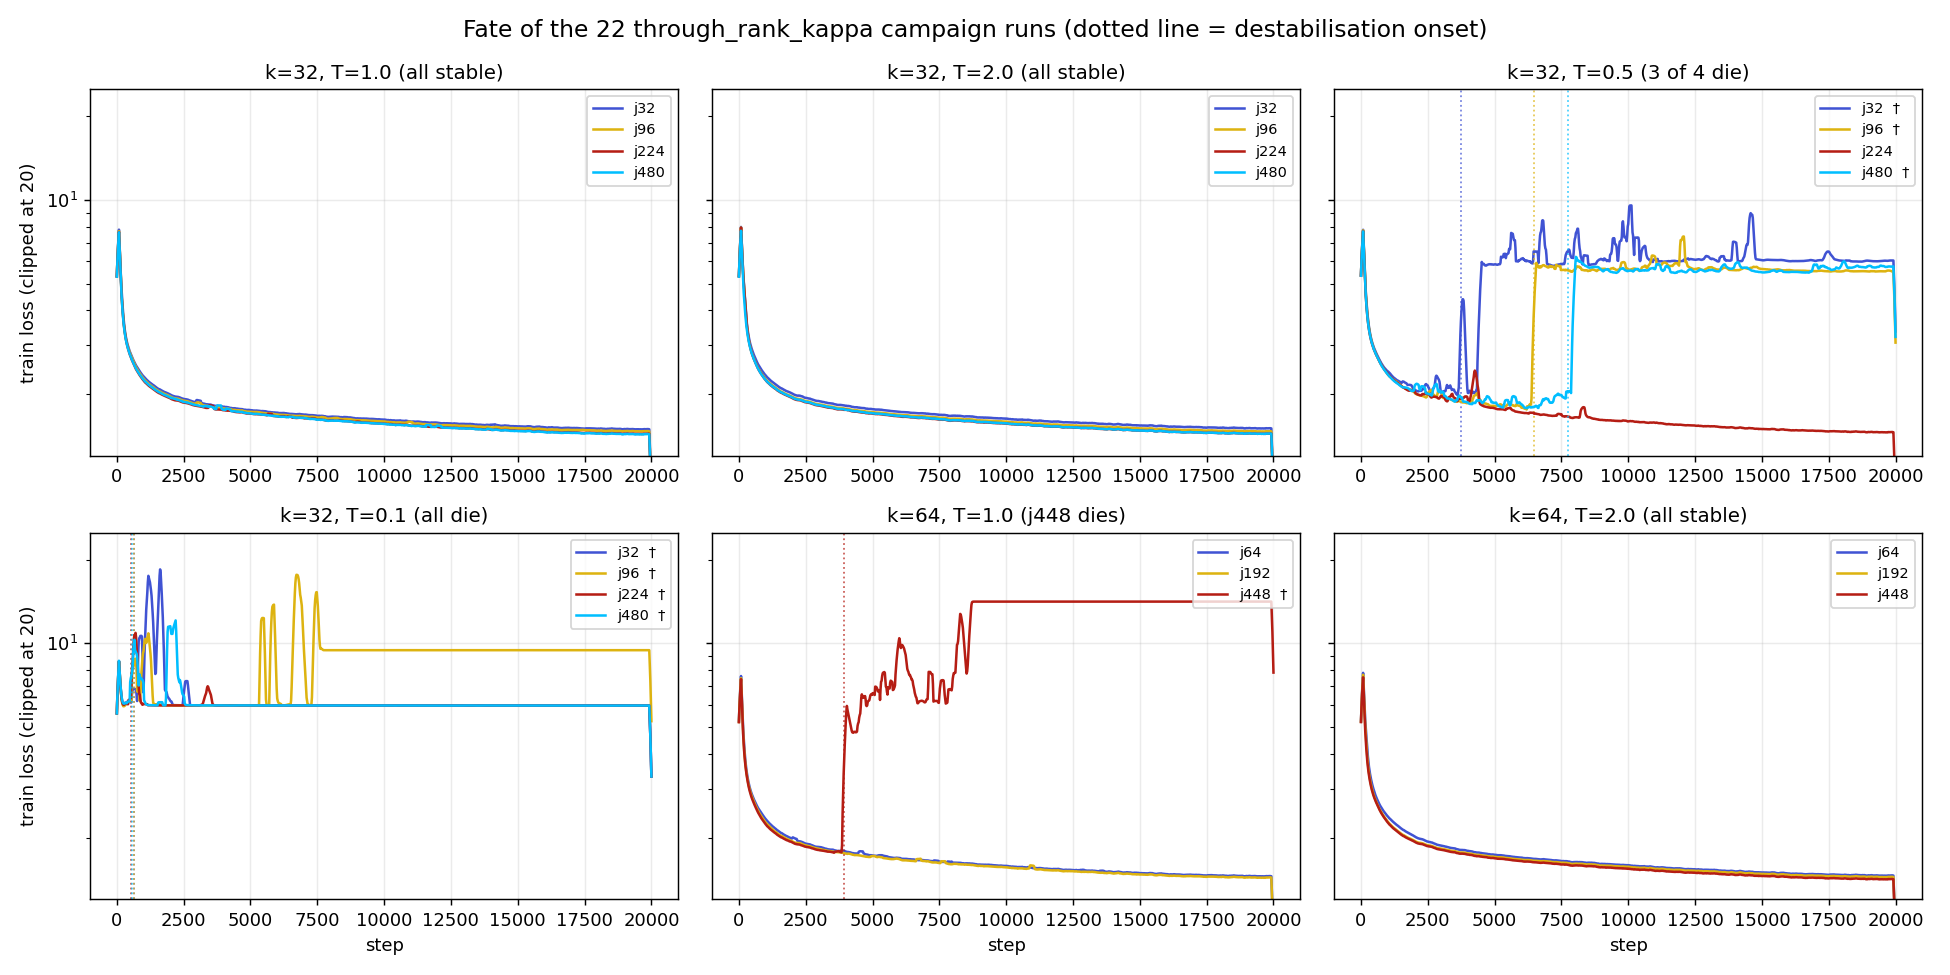
\includegraphics[width=\textwidth]{figures/kstab_fate_grid.png}
\caption{Train-loss fate grid of the 22 \code{through\_rank\_kappa} campaign
runs; dotted lines mark destabilisation onsets.}
\end{figure}

Facts the TB signals add (all runs, dying and stable):

\begin{itemize}[leftmargin=1.4em]
\item \code{rb\_cap\_active\_frac} $\equiv 1.0$ always, even mid-collapse ---
  the $b_0$ floor never engages. \textbf{H4 is dead.}
\item \code{rb\_common\_mode} stays ${\sim}10^{-6}$: the kappa correction
  stays exactly zero-sum while the run diverges. The correction operates as
  designed throughout.
\item The \textbf{boundary score inflates long before the loss reacts}: the
  $T{=}0.5$ victims carry $b$ at 25--500$\times$ baseline for
  hundreds--thousands of steps pre-onset; $k64/j448$ shows $+22\%$ $b$ and
  $4.4\times$ grad-norm in its last 1000 steps.
\item \code{rb\_support\_grad\_norm} does \emph{not} grow pre-onset --- the
  surrogate force never explodes; it quietly steers the model into an
  unstable region, and the \emph{ordinary} loss gradients blow up when the
  model arrives there.
\end{itemize}

\begin{figure}[h]\centering
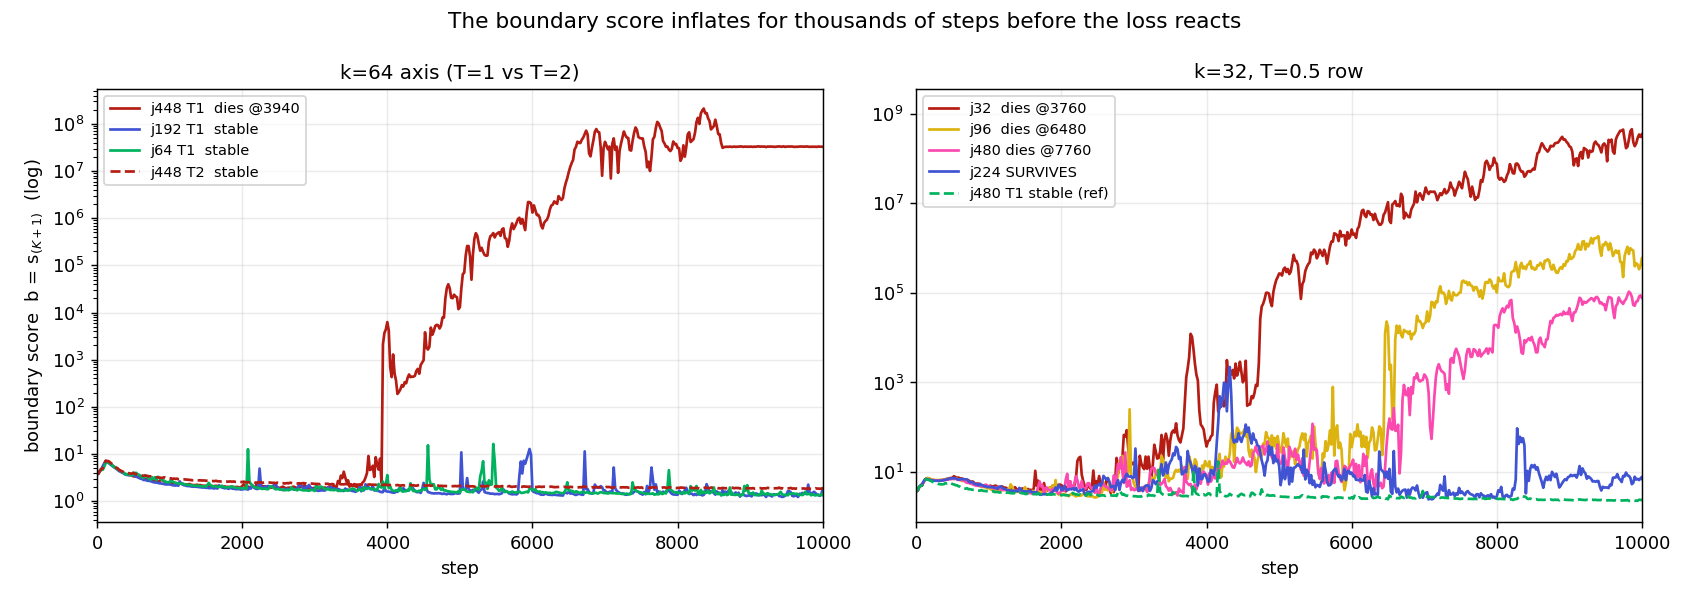
\includegraphics[width=\textwidth]{figures/kstab_boundary_inflation.png}
\caption{The boundary score inflates for thousands of steps before the loss
reacts. Left: the $k{=}64$ axis; right: the $k{=}32$, $T{=}0.5$ row.}
\end{figure}

\textbf{The figure above changed the shape of the theory.} Destabilisation is
not a smooth drift: every marginal run shows repeated \emph{inflation bursts}
--- transient boundary excursions (up to $10^3\times$) that mostly
\emph{recover}. The $T{=}0.5$ survivor ($j224$) rode out a $10^3$ burst at
${\sim}4300$ twice. Each victim's death is one burst that fails to recover and
hands over to a permanent exponential climb. Death is a noise-activated
\textbf{escape event}.

Burst census (excursions of $b$ above $3\times$ its rolling median, per 1000
steps, pre-onset only):

\begin{center}\small
\begin{tabular}{lll}
\toprule
row & burst rate & fate \\
\midrule
$k{=}32\;T{=}2$ and $k{=}64\;T{=}2$ & 0.00 & all stable (max excursion $\le1.9\times$) \\
$k{=}32\;T{=}1$ & 0.05--0.21 & all stable \\
$k{=}64\;T{=}1$ & $j64$: 0.37, $j192$: 0.42, \textbf{$j448$: 0.97} & \died{$j448$ dies} \\
$k{=}32\;T{=}0.5$ & $j224$: \textbf{0.52}, $j480$: 1.7, $j32$: 3.1, $j96$: 3.2 & \textbf{$j224$ alone survives} \\
\bottomrule
\end{tabular}
\end{center}

Burst rate predicts fate \emph{within} rows too: the $k64$ victim had the
highest rate of its row, the $T05$ survivor the lowest of its row by
3--6$\times$.

\section{Evidence phase 2: the forces, measured}

\code{analysis/kappa\_stability.py probe} reconstructs the exact surrogate
force per candidate from the probe captures ($u = \partial L/\partial\tilde z$
and signed $z$, steps 0--1000 every 10). The reconstruction matches the
captured $\partial L/\partial z$ to ${\sim}0.000$ relative error, so these are
the true training-time forces.

\textbf{The $T{=}0.1$ collapse, anatomised} ($k32\,j96$; layer 4; kick = mean
$|g_s|$ in the kernel window, $\neff$ = how many candidates share the window):

\begin{center}\small
\begin{tabular}{rrrrrr}
\toprule
step & probe CE & kick & $\neff$ & $s_{(K+1)}$ & top-$K$ mean \\
\midrule
0    & 11.30 & $7.2\cdot10^{-3}$ & 22 & 3.8 & 4.3 \\
100  & 7.18  & $5.7\cdot10^{-5}$ & 15 & 4.9 & 5.7 \\
150  & 6.20  & $1.9\cdot10^{-4}$ & 3  & 11.9 & 15.6 \\
250  & 6.10  & $6.1\cdot10^{-4}$ & 2  & 36 & 47 \\
350  & 5.84  & $1.7\cdot10^{-6}$ & \textbf{1} & 50 & 73 \\
500  & 6.06  & ${\sim}0$ & 1 & 664 & 1297 \\
1000 & 17.2  & ${\sim}0$ & 1 & 21941 & 49688 \\
\bottomrule
\end{tabular}
\end{center}

The sequence: a huge initial kick ($\kappa_{\max} = 1/(2T) = 5$) $\to$ scores
inflate to escape the kernel $\to$ the window population $\neff$ collapses to
\textbf{1} $\to$ the kappa correction \emph{degenerates into
\code{through\_rank}} (the whole zero-sum lands on one boundary feature ---
the proven-divergent mode) $\to$ runaway inflation $\to$ kernel dead (kick
$\to 0$) $\to$ the model is stranded at $10^3$--$10^4\times$ activation scale,
CE frozen ${\sim}6$. Support churn: 96\% of the top-$K$ replaced per 10 steps
at the start (vs.\ ${\sim}30\%$ healthy), then frozen solid (overlap
$\to 1.0$).

\textbf{The pressure number.} Define the \emph{kick-to-spacing ratio}
\[
  \chi \;=\; \frac{\overline{|g_s|}_{\,\text{window}}}{\delta(b)}
\]
(how far one surrogate kick moves a boundary score, relative to the score
distance between neighbouring ranks there --- $\chi \gtrsim 1$-ish per
\emph{optimizer step} would mean ranks reshuffle every step; the raw
gradient-unit values below are much smaller but comparable across runs).
Measured at steps 300--1000:

\begin{center}\small
\begin{tabular}{lll}
\toprule
row & $\chi$ (layer-mean) & fate \\
\midrule
$k{=}32\;T{=}2$ & $2.7\cdot10^{-5}$ & stable \\
$k{=}64\;T{=}2$ & $5.4\cdot10^{-5}$ & stable \\
$k{=}32\;T{=}1$ & $8.2\cdot10^{-5}$ & stable \\
$k{=}64\;T{=}1$ & $1.5$--$1.7\cdot10^{-4}$ (all three $j$!) & marginal: 1 of 3 dies \\
$k{=}32\;T{=}0.5$ & $1.9\cdot10^{-4}$ & marginal: 3 of 4 die \\
$k{=}32\;T{=}0.1$ & ${\sim}10^{-2}$ at init & dies in ${\sim}150$ steps \\
\bottomrule
\end{tabular}
\end{center}

$\chi$ is a \emph{row} property (nearly identical across $j$ at fixed $k,T$)
and cleanly orders the rows: \textbf{safe below ${\sim}10^{-4}$, marginal at
${\sim}1.5$--$2\cdot10^{-4}$, instant death at ${\sim}100\times$ that.} The
user's hunch is confirmed: the $k$-axis failure and the $T$-axis failure are
the same mechanism, because
\[
  \chi \;\propto\; \frac{|u|\; b}{2\,T\,\delta(b)},
\]
and the rank-65 boundary lives in a ${\sim}3.3$--$4.6\times$ denser score
region ($\delta_{33}/\delta_{65}$ measured in \emph{the same tensors} of every
healthy model) at ${\sim}30\%$ lower $b$, giving
\[
  \frac{\chi(k{=}64,\,T{=}1)}{\chi(k{=}32,\,T{=}1)} \;\approx\; 2.2
  \;\approx\; \frac{\chi(k{=}32,\,T{=}0.5)}{\chi(k{=}32,\,T{=}1)}.
\]
Equivalently: \textbf{$k{=}64$ at $T{=}1$ IS $k{=}32$ at $T{\approx}0.5$.} The
measured safe-$T$ ratio $T_c(64)/T_c(32) \approx 2.2$ matches the campaign
outcome ($T{=}2$ safe at $k{=}64$).

Two side-findings:
\begin{itemize}[leftmargin=1.4em]
\item $\neff$ at healthy steady state is 46--446 --- nowhere near 1. The kappa
  correction only degenerates \emph{during} bursts/collapses. H1 as a standing
  explanation is dead; it survives as the \emph{cliff} at the end of a burst.
\item The per-feature ratchet is real but tiny in healthy runs: window members
  kicked up fall ${\sim}0.04$ score units less per 10 steps than members
  kicked down, on a mean regression flow of $-0.5$. The surrogate is a
  2--5\% bias on the natural score dynamics --- consistent with ``quiet
  steering'', not ``domination''.
\end{itemize}

\section{Theory v3: burst-escape}

\begin{enumerate}[leftmargin=1.6em]
\item The kernel exerts pressure $\chi$ on the boundary region. The model's
  cheapest response (norm-pinned MD weights, downstream norms) is to inflate
  its score scale, which sheds window members; the CE loss pushes back.
\item At safe $\chi$ the tug-of-war equilibrates (zero bursts at $T{=}2$, tiny
  rare bursts at $k32/T1$). At marginal $\chi$ the equilibrium is punctuated
  by stochastic inflation bursts.
\item A burst that transiently empties the window ($\neff \to O(1)$) flips the
  kappa correction into its \code{through\_rank}/point-sink degenerate limit
  --- which is \emph{itself} an inflation pump --- the burst becomes
  self-sustaining, the kernel dies entirely, and the network is stranded at
  enormous activation scale (frozen CE $\approx 6$, or worse once numerics
  saturate).
\item $T{=}0.1$ reaches the cliff deterministically in ${\sim}150$ steps;
  marginal rows reach it stochastically (burst roulette, onset 3.7--7.7k,
  victim = highest burst rate); safe rows never reach it.
\end{enumerate}

\section{Falsification wave 1 (6k steps, 20k schedules)}

Pre-registered predictions:

\begin{center}\small
\begin{tabular}{p{3.6cm}p{4.4cm}p{5.6cm}}
\toprule
run & tests & prediction (v3) \\
\midrule
$k64\,j448\,T1$ \textbf{detach} & is the kappa correction the cause? & v3 says
the \emph{raw} kernel force is the pump; detach at this pressure should die
too \\
$k64\,j448\,T1$ \textbf{project} & uniform vs.\ $\kappa$-weighted zero-sum &
should be between detach and kappa \\
$k64\,j448\,T1$ seed 1338 & is the 3940 death deterministic? & dies again, at
a different step (burst roulette) \\
$k64\,j448$ \textbf{$T{=}1.5$} & $\chi$ threshold bracket
($\chi \approx 1.0$--$1.1\cdot10^{-4}$) & at the safe edge: survives 6k,
marginal at 20k \\
$k64$ \textbf{$j320$} $T1$ & $j$-threshold inside the marginal row & same
$\chi$ as siblings $\Rightarrow$ survival decided by burst luck; rate between
$j192$ and $j448$ \\
$k32\,j480$ \textbf{$T{=}0.75$} & $\chi$ bracket on the $k32$ axis
($\chi \approx 1.1\cdot10^{-4}$) & marginal-safe: survives 6k \\
$k32\,j96\,T05$ seed 1338 & victim reshuffle & dies, at a different onset than
6480 \\
probe5k of $k64\,j448\,T1$ & gradient-resolved capture through the death &
$\neff \to O(1)$ during the fatal burst; $\chi$ flat-then-spike, not a slow
ramp \\
\bottomrule
\end{tabular}
\end{center}

\textbf{Early returns (step ${\sim}1100$):} detach CE 9.0 with
grad-norm $=\infty$ and project CE 7.1 with grad-norm $=\infty$ --- both
already collapsed, while every kappa run is healthy at the same step. At
$k32/T1$ detach had been stable for 20k. So the correction is not the villain
--- it is the \emph{strongest} of the three modes at this pressure (kappa
outlived detach $4\times$), and what kills it is the burst that transiently
strips its window. Consistent with v3.

\begin{figure}[h]\centering
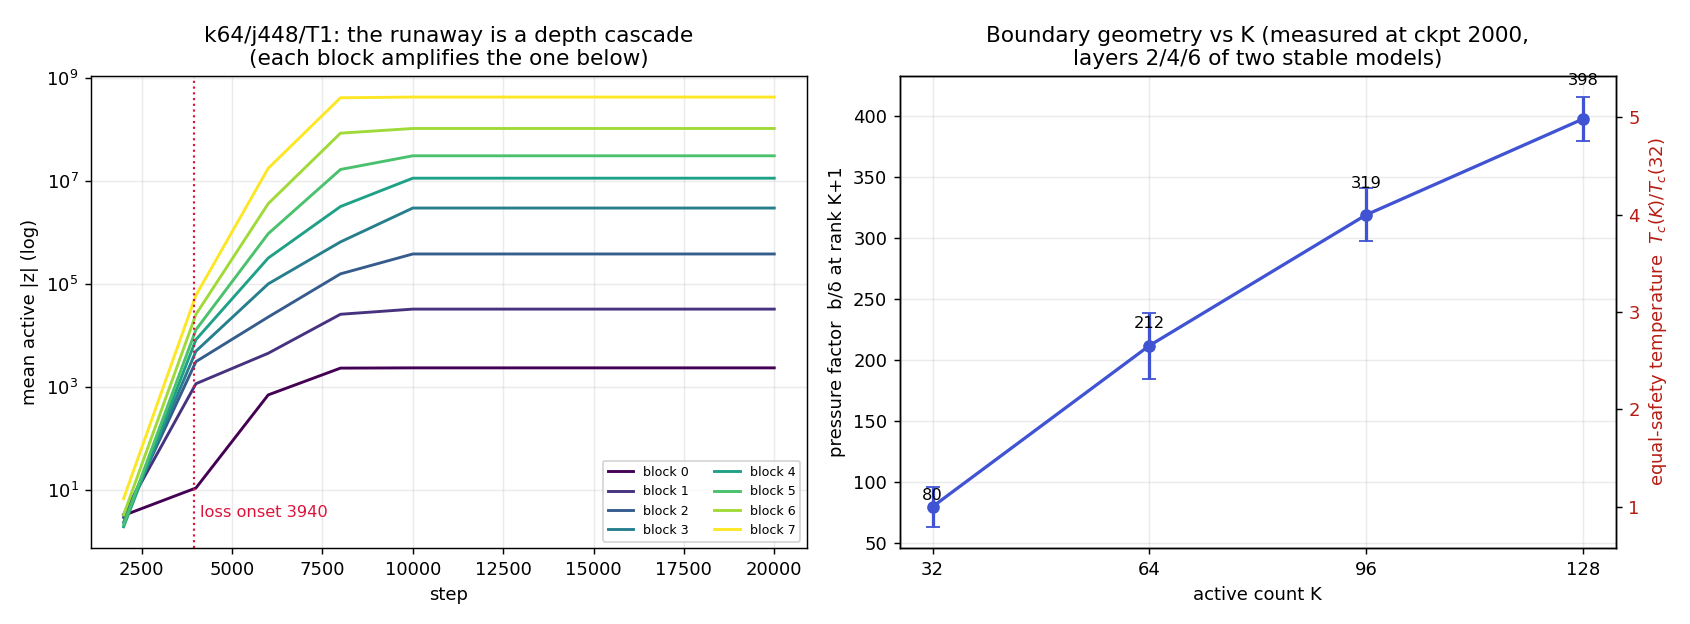
\includegraphics[width=\textwidth]{figures/kstab_cascade_and_geometry.png}
\caption{Left: once past the point of no return the inflation is a clean depth
cascade --- each block amplifies the scale handed up by the one below
(\code{residual\_out} replaces the residual, so scale multiplies through
depth), ending in bf16-saturation plateaux. Right: the pressure factor
$b/\delta$ grows near-linearly with $K$ --- this is why ``just pick a bigger
fixed $T$'' always fails eventually.}
\end{figure}

\begin{figure}[h]\centering
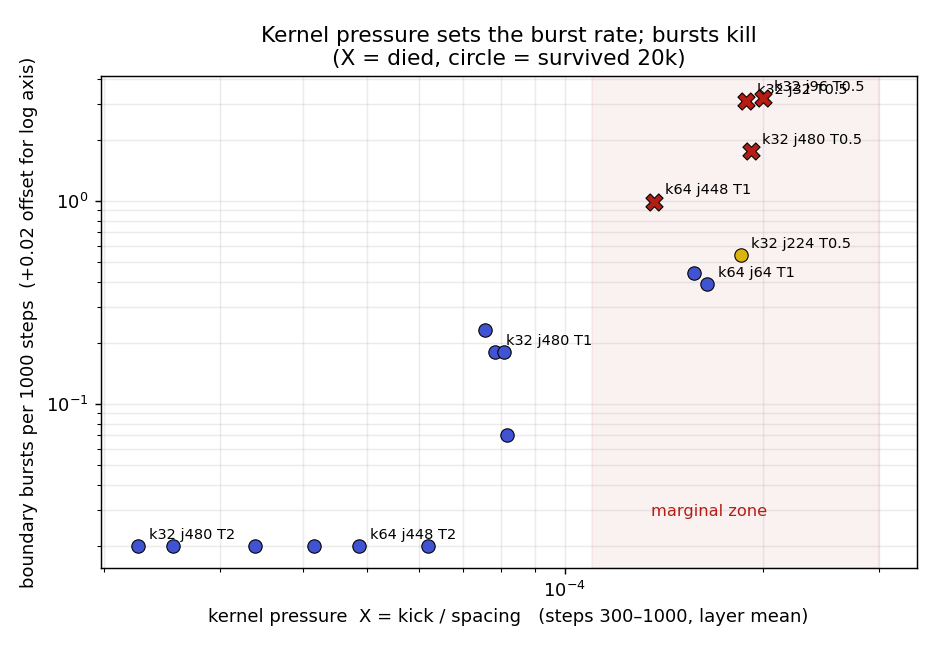
\includegraphics[width=.72\textwidth]{figures/kstab_dose_response.png}
\caption{Kernel pressure $\chi$ sets the burst rate; bursts kill
(cross = died, circle = survived 20k).}
\end{figure}

\begin{figure}[h]\centering
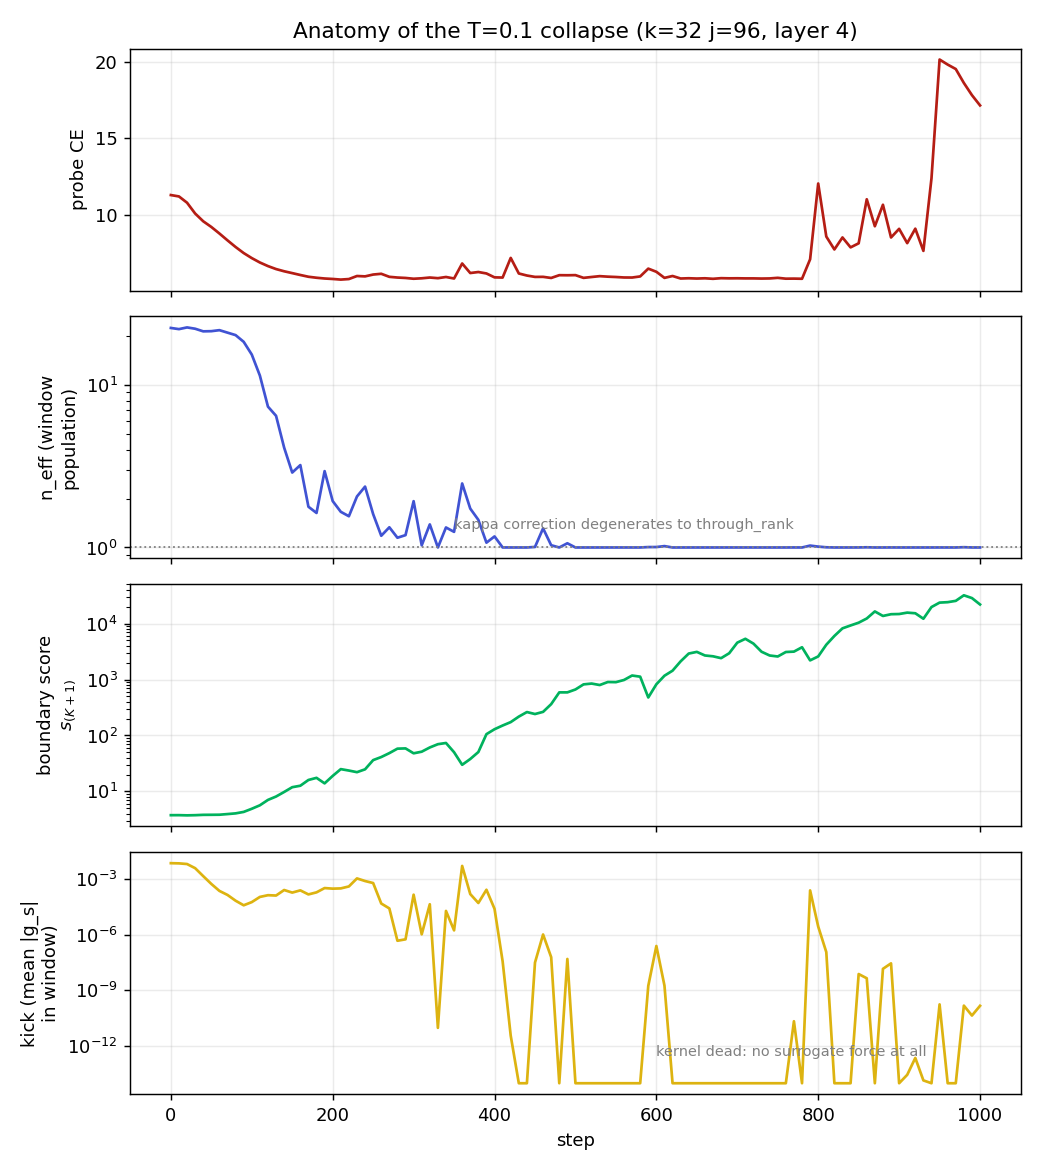
\includegraphics[width=.8\textwidth]{figures/kstab_t01_anatomy.png}
\caption{Anatomy of the $T{=}0.1$ collapse ($k{=}32$, $j{=}96$, layer 4).}
\end{figure}

The anatomy figure shows the causal order within one collapse: the window
population $\neff$ falls to 1 (step ${\sim}350$) \emph{while CE is still
fine}; the boundary score is already climbing exponentially; the kick dies as
the kernel loses everyone (step ${\sim}450$); CE only breaks visibly at
${\sim}800$. Loss is the last thing to know.

\section{The recipe: a temperature servo}

The theory says the failure needs two things: sustained kernel pressure $\chi$
above ${\sim}10^{-4}$ (sets burst rate), and a burst that empties the window
(the cliff). Both are properties the gate can \emph{measure about itself}, so
the principled fix is feedback rather than a fixed-$T$ schedule or a
$k$-lookup table:

\textbf{\code{rblapsum\_temperature\_mode:\ servo}} (implemented in
\code{src/wsparse/bottleneck/\{gate,rblapsum\}.py}, per-layer scalar $T$,
state in persistent buffers):

\begin{enumerate}[leftmargin=1.6em]
\item \textbf{Population floor} (the cliff guard): if fewer than
  \code{rblapsum\_window\_floor} $= 16$ candidates sit inside the kernel
  window on a batch, $T$ grows 10\% \emph{that step}. A window that cannot
  empty cannot hand the zero-sum correction to a single feature, so the
  \code{through\_rank} degenerate limit --- the runaway engine in every
  observed death --- becomes unreachable. During a burst the boundary runs,
  the window thins, and the servo chases it up within tens of steps
  ($1.1^{\,n}$ compounding).
\item \textbf{Kick-to-spacing trim} (the operating point): otherwise $T$ moves
  at most 2\%/step to hold $\EMA(\text{kick})/\EMA(\delta)$ at
  \code{rblapsum\_chi\_target} $= 8\cdot10^{-5}$ --- the measured $k32/T1$
  point, which is simultaneously the best-quality and the calmest stable
  configuration. This automatically delivers $T \approx 1$ at $k{=}32$,
  $T \approx 2^{+}$ at $k{=}64$, and whatever $k{=}96^{+}$ needs, with no
  manual sweep.
\end{enumerate}

Why not simpler rules that were considered and rejected:
\begin{itemize}[leftmargin=1.4em]
\item \emph{$T$ proportional to the local band spread} is scale-invariant
  (good under inflation) but moves the \textbf{wrong way in $k$}: the $k{=}64$
  boundary region is denser, so spread-following would \emph{lower} $T$ where
  more $T$ is needed.
\item \emph{A fixed $T{=}2$ everywhere} works for $k \le 64$ but the pressure
  grows with $k$ (measured $b/\delta$: $80 \to 212 \to 319 \to 398$ for
  $K = 32/64/96/128$), so any fixed choice fails at some $k$ --- and overpays
  quality at small $k$.
\end{itemize}

\section{Wave 2 (pre-registered)}

Geometry measured at checkpoint-2000 of two stable campaign models
\emph{before} these runs ($b/\delta$ above) fixes the predictions:

\begin{center}\small
\begin{tabular}{p{4.6cm}p{9.2cm}}
\toprule
run & prediction \\
\midrule
\code{kstab\_k96\_j416\_t1} (fixed $T{=}1$) & $\chi \approx 1.5\times$ the
level that killed $k64/j448$ $\to$ \died{dies}, onset earlier than 3940
(roughly 1.5--6k; death probability ${\sim}0.8^{+}$) \\
\code{kstab\_k96\_j416\_servo} & survives 20k; settled $T$ above the $k64$
servo's settled $T$ \\
\code{kstab\_k64\_j448\_servo} (+ seed 1338) & survives past 3940 both seeds;
final CE $\approx$ the $T{=}2$ twin's 1.472 or better \\
\code{kstab\_k32\_j480\_t05\_servo} ($T_0{=}0.5$) & rescued: servo lifts $T$
out of the marginal zone; final CE $\approx 1.49$ \\
\code{kstab\_k32\_j96\_t01\_servo} ($T_0{=}0.1$) & rescued from the 150-step
collapse by the population guard ($T$ must climb ${\sim}10\times$ within
${\sim}100$ steps) \\
\code{kstab\_k32\_j480\_servo} ($T_0{=}1.0$) & null test: servo holds
$T \approx 1$, quality matches the 1.491 flagship \\
\bottomrule
\end{tabular}
\end{center}

\subsection*{7b. What the force looks like rank-by-rank (and one honest
unknown)}

\emph{(Addendum to \S7, recorded after \S11.)} Reconstructed per-rank means
over steps 300--1000 ($k{=}64/T{=}1$ probes, layer 4): the surrogate force is
a \textbf{dipole centred on the boundary} --- the \emph{marginal actives}
(ranks ${\sim}33$--64) carry $w < 0$ (the loss wants them weaker) and get
pushed down; the near-tail (65--128) gets pushed up; the top-16, which the
loss genuinely wants stronger ($w \approx +9\cdot10^{-7}$, the largest in the
table), barely feels the kernel ($\kappa \approx 0.05$). So in its healthy
regime the gate runs a \emph{swap pump}: it actively closes the gap and
encourages the support to exchange marginal members for promising tail
members. That is the mechanism working as intended --- the pathology is only
its interaction with a too-sharp kernel.

Two more within-row facts:
\begin{itemize}[leftmargin=1.4em]
\item The \emph{uncorrected} common-mode total $\sum_i a_i$ is
  4--5$\times$ \textbf{larger} at $j{=}64$ than at $j{=}448$ (a truncated tail
  cancels less), yet $j{=}64$ is the stable one --- more evidence that the
  kappa correction neutralises the common mode exactly and the common mode is
  not the driver.
\item At $T{=}1$ the kernel reaches the whole candidate set even at $j{=}448$
  ($\kappa \approx 0.18$ at rank 512), so $j$ sets the \emph{window
  population} ($\neff = 102/206/373$ for $j = 64/192/448$). Within the
  $k{=}64$ row, burst rate tracks population ($0.37/0.42/0.97$ per 1k).
  \textbf{Open residual:} the $T{=}0.5$ row does \emph{not} follow the same
  ordering ($j32$ has the smallest window and the most bursts), so the
  within-row victim selection at $T{=}0.5$ is not explained by population
  alone --- plausibly threshold-saturated chaos; the seed-repeat runs speak to
  this.
\end{itemize}

\section{Wave 1 results (6k steps, 20k schedules)}

\begin{center}\small
\begin{tabular}{p{2.9cm}p{3.1cm}p{4.2cm}p{3.4cm}}
\toprule
run & predicted & observed & verdict \\
\midrule
$k64\,j448\,T1$ \textbf{detach} & dies (raw force is the pump) & died
\textbf{inside the first 100 steps} (frozen CE 9.06) & \ok\ok\ --- even faster
than kappa's 3940 \\
$k64\,j448\,T1$ \textbf{project} & between detach and kappa & died $<100$
steps (frozen CE 7.09) & \ok\ (uniform mean-removal $\approx$ no protection
here) \\
$k64\,j448\,T1$ \textbf{seed 1338} & dies at a different step &
\textbf{survived 6k} (1.687), bursting at the row rate 0.39/1k & \fail\ on
the letter --- \ok\ on the substance: with the probe5k replica also surviving
to 4800, 2 of 3 trajectories of the killer config live past 4k. Death is a
stochastic escape, not a deterministic event \\
$k64\,j448$ \textbf{$T{=}1.5$} & edge of safe: survives 6k & survived,
\textbf{zero bursts} (max excursion $1.5\times$) & \ok, calmer than
predicted \\
$k64$ \textbf{$j320$} $T1$ & roulette at row rate & survived, 0.39 bursts/1k
& \ok \\
$k32\,j480$ \textbf{$T{=}0.75$} & safe edge & survived (1.730), 0.19
bursts/1k & \ok \\
$k32\,j96\,T05$ \textbf{seed 1338} & dies at a different onset & died, onset
\textbf{3680} (seed 1: 6480), one $10^6\times$ burst & \ok \\
probe5k through-death capture & $\neff \to O(1)$ during the fatal burst & no
death this time --- but two discoveries below & partial \\
\bottomrule
\end{tabular}
\end{center}

Two refinements from the gradient-resolved replica (figure below):

\begin{figure}[h]\centering
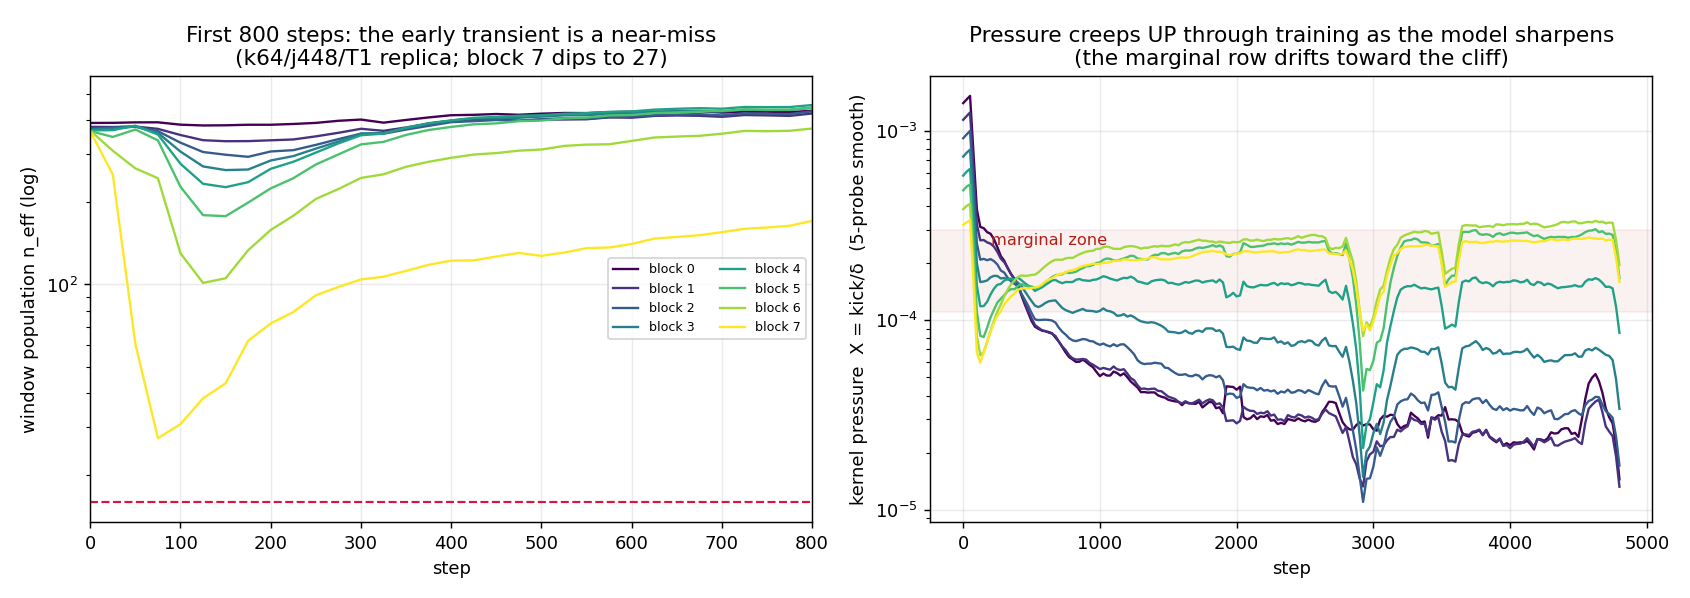
\includegraphics[width=\textwidth]{figures/kstab_probe5k_dip_creep.png}
\caption{Gradient-resolved replica of $k64/j448/T1$. Left: the early
transient's window-population dive. Right: kernel pressure creeps upward
through training.}
\end{figure}

\begin{itemize}[leftmargin=1.4em]
\item \textbf{The early transient is a near-miss.} In the first ${\sim}100$
  steps the deep blocks' window population crashes (block 7: $363 \to 27$)
  while $\chi$ starts at ${\sim}10^{-3}$. This is exactly when $T{=}0.1$,
  detach and project die. Everything that survives does so by squeaking
  through this phase.
\item \textbf{Pressure creeps upward through training.} After recovery,
  $\chi$ climbs steadily (block 7: $1.2\cdot10^{-4} \to 2.7\cdot10^{-4}$ by
  step 4800) because the sharpening score geometry shrinks $\delta$ faster
  than the kick decays. Marginal rows drift deeper into burst territory with
  time --- late stochastic deaths (3.7--7.7k) are not just waiting for a rare
  burst; the burst rate itself grows. A fixed $T$ must be sized for the worst
  moment of the worst layer; a feedback $T$ pays only where and when pressure
  exists.
\item \textbf{The pressure is layer-heterogeneous}: blocks 5--7 live in the
  marginal zone, blocks 0--4 relax to safe levels --- the servo being
  per-layer is not an implementation detail but a requirement.
\end{itemize}

Theory status after wave 1: no surviving contradiction. The one falsified
letter-prediction (seed 1338 ``dies again'') sharpened the claim: \textbf{a
marginal row sets a death \emph{rate}, not a death sentence} --- consistent
with the \code{through\_rank} regen that also refused to re-diverge.

\section{Wave 2.0 aborted by its own telemetry --- the trim redesigned}

800 steps into the first servo wave the telemetry showed the kick-based trim
mis-calibrated: healthy runs were trimming $T$ \emph{down} ($k64$:
$0.97 \to 0.45$) onto the population floor, because measured live chi sat far
below the $8\cdot10^{-5}$ target. Root cause: \textbf{the kick $|g_s|$
carries the training loss's per-token normalisation} --- the probe captures
that calibrated the target use 256-token batches, live steps use ${\sim}50$k
tokens, so a gradient-unit threshold is off by that ratio. Gradient-unit
targets do not transfer. (The $T_0{=}0.1$ rescue was nevertheless already
working --- the floor guard had lifted $T$ to 0.5 with healthy loss while
fixed-$T{=}0.1$ was long dead.)

The fix drops gradient units entirely. Checking the fate table against the
\textbf{pure-geometry pressure}
\[
  \chigeo \;=\; \frac{b}{2\,T\,\delta}
\]
--- forward-only, dimensionless --- measured at ckpt 2000 (layer max): every
run that stayed $\le{\sim}55$ survived; every death carried $\ge{\sim}58$; the
$k64/T1$ row sits at ${\sim}114$ where survival is seed roulette. The
$u$-factor evidently contributes little discriminating signal on top of the
geometry. The servo's trim now holds
\[
  \chigeo \;=\; \frac{\EMA(b)}{2\,T\,\EMA(\delta)}
\]
at 45, just below the proven $k32/T1$ operating point (${\sim}51$); the
population floor stays as the burst backstop.

Wave 2.1 relaunched (same six runs, same names). Sharpened, falsifiable
settling predictions from $\chigeo^{*} = 45$ and the measured
$b/\delta \approx 80/212/319$ at $K = 32/64/96$: \textbf{the servo should
settle $T \approx 0.9$--$1.2$ at $k{=}32$, $\approx 2$--$2.6$ at $k{=}64$,
$\approx 3$--$4$ at $k{=}96$} (deep blocks highest), discovering the entire
$T_c(K)$ line on its own --- with $k32$/$k64$ quality matching the fixed-$T$
flagships (1.491 / 1.472).

\section{Wave 2.1 mid-flight (step ${\sim}2400$) --- the servo settles where
predicted}

\begin{center}\small
\begin{tabular}{lrrrrrl}
\toprule
run & $T_0$ & \code{rb\_temp} @2.4k & \code{rb\_chi} & window & loss &
pre-registered $T$ \\
\midrule
\code{k32\_j480\_servo} & 1.0 & \textbf{0.947} & 46.4 & 129 & 1.919 &
0.9--1.2 \ok \\
\code{k32\_j480\_t05\_servo} & 0.5 & \textbf{0.946} & 37.2 & 143 & 1.942 &
(rescue) $\to$ same point \ok \\
\code{k32\_j96\_t01\_servo} & 0.1 & \textbf{1.039} & 44.8 & 103 & 1.905 &
(rescue from the 150-step killer) \ok\ok \\
\code{k64\_j448\_servo} & 1.0 & \textbf{2.268} & 45.0 & 450 & 1.884 &
2--2.6 \ok \\
\code{k96\_j416\_servo} & 1.0 & \textbf{3.001} & 45.5 & 483 & 1.908 &
3--4 \ok \\
\bottomrule
\end{tabular}
\end{center}

Three different starting temperatures at $k{=}32$ (1.0, 0.5, 0.1 --- one safe,
one usually-lethal, one always-lethal) converge onto the same
${\approx}0.95$--1.04: the controller's operating point is well-defined and
path-independent. The servo has effectively \emph{discovered the $T_c(K)$
line by itself} ($0.95 / 2.27 / 3.00 \approx$ proportional to the measured
$b/\delta = 80/212/319$), while every loss sits on the healthy fixed-$T$
trajectory.

Meanwhile \textbf{\code{kstab\_k96\_j416\_t1} (fixed $T{=}1$) died on
schedule} --- loss $\approx 6.0$ by step 3800, inside the pre-registered
1.5--6k window. That is the theory's sharpest confirmed prediction: a
never-tried $K$, called in advance from score geometry alone.

\section{Wave 2.1 results (20k): four hits, two rescues --- and the null test
failed}

\begin{center}\small
\begin{tabular}{p{4.4cm}p{3.6cm}rp{4.2cm}}
\toprule
run & fate & final CE & reference \\
\midrule
\code{kstab\_k64\_j448\_servo} & stable & \textbf{1.4691} & fixed $T{=}2$:
1.4724; fixed $T{=}1$: died 3940 \\
\code{kstab\_k64\_j448\_servo\_s2} & stable & \textbf{1.4608} & best $k{=}64$
result of the project \\
\code{kstab\_k96\_j416\_servo} & stable & \textbf{1.4734} & fixed $T{=}1$:
died at 1640 --- $k{=}96$ had never trained \\
\code{kstab\_k32\_j480\_t05\_servo} ($T_0{=}0.5$) & stable (one survived burst
@${\sim}8.9$k) & 1.5075 & fixed $T{=}0.5$: died 7760 \\
\code{kstab\_k32\_j96\_t01\_servo} ($T_0{=}0.1$) & stable (one survived burst
@${\sim}5.1$k; guard visibly spiked $T$ to 2.2 and rode it out) & 1.5261 &
fixed $T{=}0.1$: dead in 640 steps; fixed $T{=}1$ same $j$: 1.525 \\
\textbf{\code{kstab\_k32\_j480\_servo}} ($T_0{=}1$, the null test) &
\died{destabilised @4140} & 3.945 & fixed $T{=}1$: 1.491 stable \\
\bottomrule
\end{tabular}
\end{center}

\begin{figure}[h]\centering
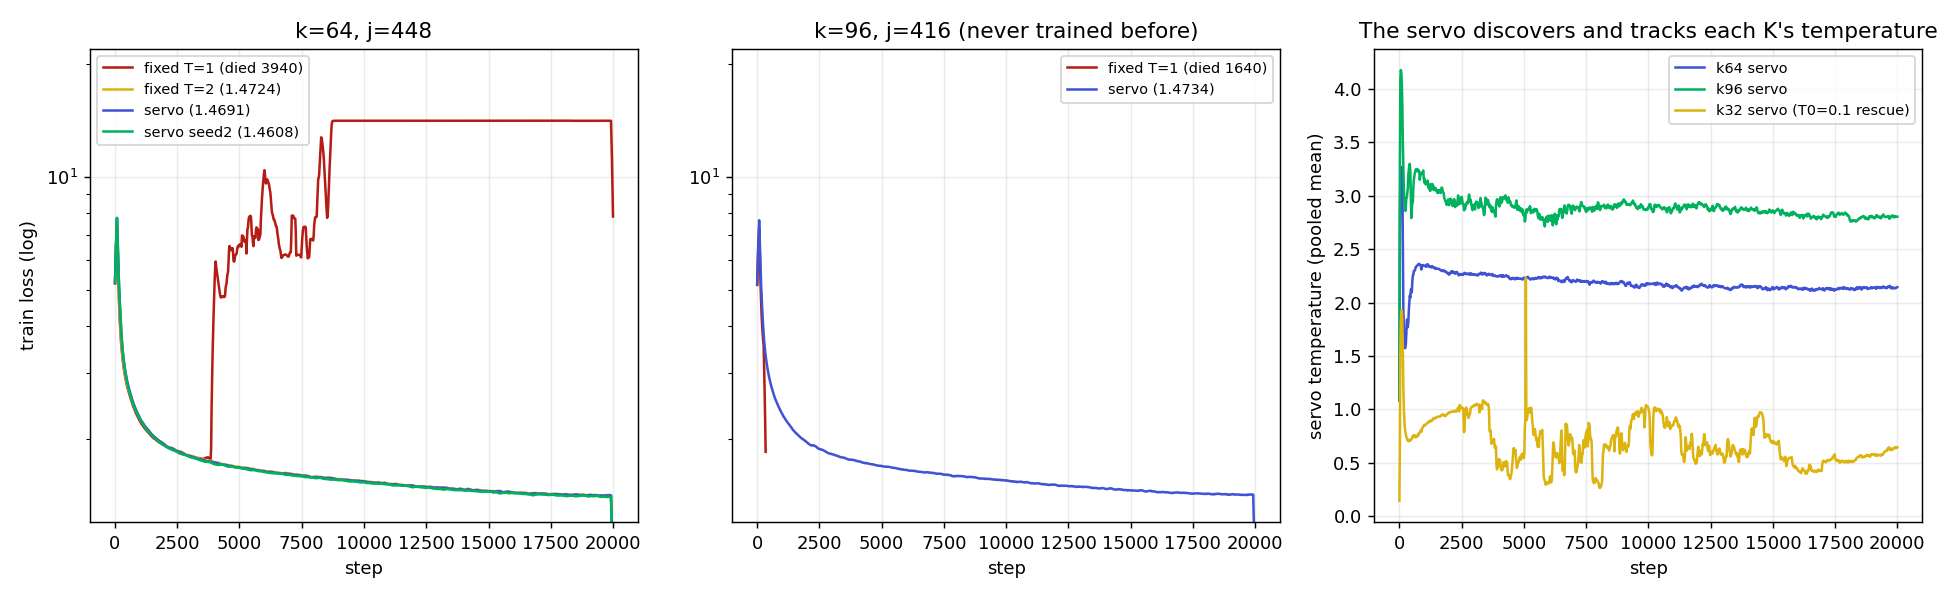
\includegraphics[width=\textwidth]{figures/kstab_servo_headline.png}
\caption{Servo vs.\ fixed temperature. Left: $k{=}64$, $j{=}448$; middle:
$k{=}96$, $j{=}416$; right: the temperatures the servo discovers and tracks.}
\end{figure}

\textbf{The null-test failure is the most instructive result of the wave.}
Post-mortem (left panel below): the symmetric trim, holding $\chigeo = 45$,
walked $T$ \emph{down} to 0.49--0.70 by steps 4--8k --- inside the
proven-marginal $T \approx 0.5$--0.75 band --- because the safe operating line
is not a constant: the stable fixed $k32/T1$ flagship runs at
$\chigeo \approx 39$ falling to ${\sim}30$ over training (right panel).
Holding 45 therefore means \emph{sharpening beyond the proven-safe point
exactly where the geometry is calmest}. The boundary inflated silently for
thousands of steps, and a late giant burst ($b \to 2500$) outran the guard.
Meanwhile the two $k32$ runs that started from lethal temperatures survived
--- the $k32$ servo family was collectively operating in the marginal band
and the roulette picked the null test. A cruel but perfect demonstration of
the theory's own dose--response claim.

\begin{figure}[h]\centering
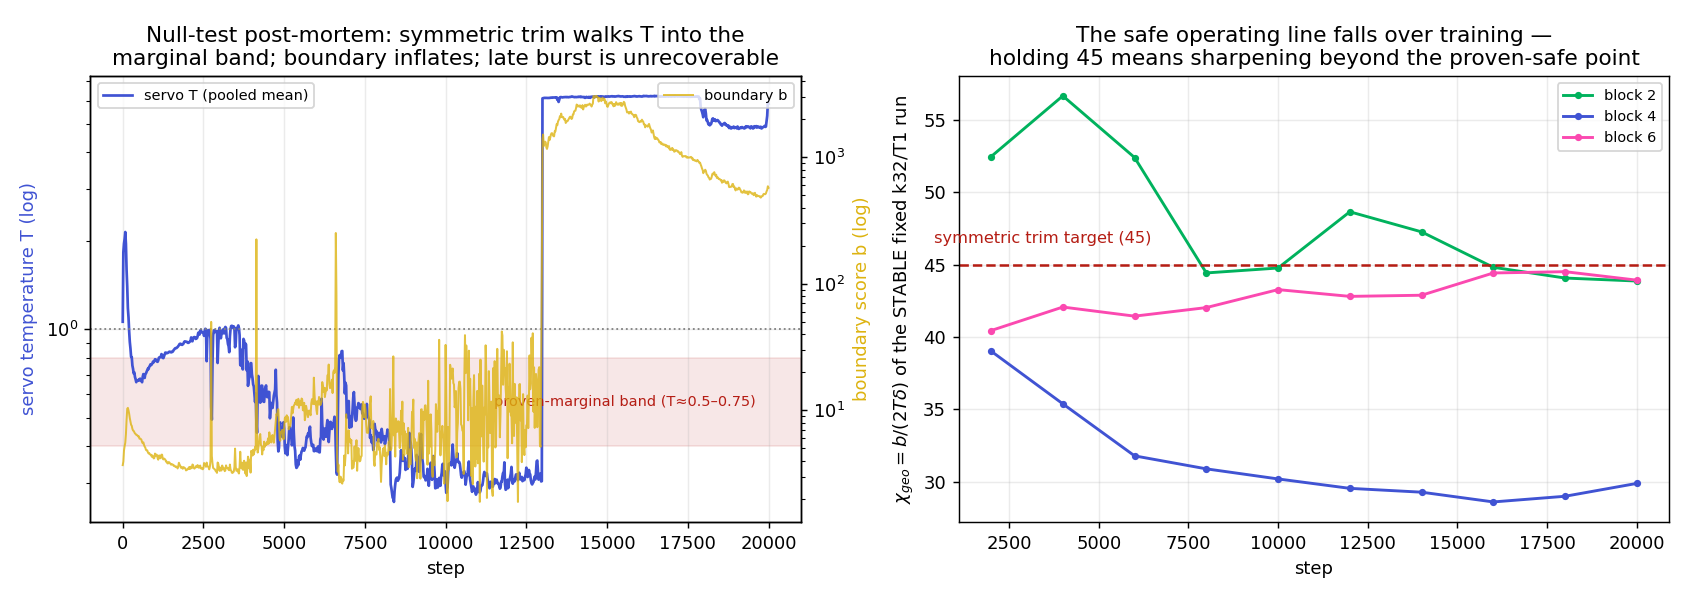
\includegraphics[width=\textwidth]{figures/kstab_nulltest_postmortem.png}
\caption{Null-test post-mortem. Left: the symmetric trim walks $T$ into the
marginal band; the boundary inflates; the late burst is unrecoverable. Right:
the stable fixed $k32/T1$ run's $\chigeo$ falls over training --- holding 45
means sharpening beyond the proven-safe point.}
\end{figure}

\textbf{Fix (implemented, tested): the trim is now protective-only} --- $T$
never goes below the configured \code{rblapsum\_temperature}. The servo's
mandate is asymmetric by nature: rising above the baseline prevents deaths
(proven at $k{=}64$/96); dipping below it only chases quality that the fixed
baseline already delivers, at documented risk. Wave 2.2 (running): the null
test redone under the protective floor (two seeds) plus a $k{=}96$ seed
repeat.

\textbf{Per-layer temperatures the servo discovered} (final checkpoints,
blocks $0 \to 7$): $k64$: 2.74, 2.48, 2.11, 1.83, 1.82, 1.99, 1.97, 2.21 ---
a U over depth (first and last blocks sharpest-geometried); $k96$ the same
shape one size up (3.52 \dots\ 2.06 \dots\ 3.06). A ${\sim}1.5\times$ spread
inside one model: per-layer control is not an implementation nicety, no
single scalar $T$ is right for all blocks.

\section{Wave 2.2 (20k, protective-only trim): the null test passes}

\begin{center}\small
\begin{tabular}{p{4.6cm}p{3.0cm}rp{4.2cm}}
\toprule
run & fate & final CE & reference \\
\midrule
\code{kstab\_k32\_j480\_servo} (redo) & stable, no onset & \textbf{1.4879}
& fixed $T{=}1$: 1.4910; symmetric-trim version: died @4140 \\
\code{kstab\_k32\_j480\_servo\_s2} & stable, no onset & 1.4957 & seed
robustness \\
\code{kstab\_k96\_j416\_servo\_s2} & stable, no onset & \textbf{1.4665} &
seed 1: 1.4734; fixed $T{=}1$: died @1640 \\
\bottomrule
\end{tabular}
\end{center}

The protective floor fixes the one failure of wave 2.1 --- and the redo not
only matches the fixed-$T{=}1$ flagship, it edges past it.

\section{Final answers}

\textbf{What destabilizes \code{through\_rank\_kappa}?} Kernel pressure on
the boundary neighbourhood: when the kernel is too sharp for the local score
geometry (too few ``rungs'' of the score ladder inside the window, each
feeling too strong a kick), the model responds by inflating its score scale,
in stochastic bursts. A burst that empties the window ($\neff \to 1$) flips
the kappa correction into \code{through\_rank}'s point-sink limit --- the
proven runaway engine --- and the burst becomes self-sustaining:
depth-cascading activation inflation, kernel death, terminal collapse. The
zero-sum correction itself never fails; it is the most protective of the
three modes (detach and project die $40\times$ faster at the same pressure).

\textbf{Are the $k$-axis and $T$-axis failures the same mechanism?} Yes.
Both axes move one dimensionless number, the geometric pressure
$\chigeo = b/(2T\delta)$: raising $k$ moves the boundary into a denser part
of the score distribution ($b/\delta \approx 80 \to 212 \to 319 \to 398$
at $K = 32/64/96/128$), lowering $T$ sharpens the kernel. Measured
equivalence: $k{=}64$ at $T{=}1$ $\approx$ $k{=}32$ at $T{\approx}0.5$ ---
and both sat in the same marginal band with the same burst phenomenology.
The $k{=}96$ death at fixed $T{=}1$ was called in advance (onset window and
all) from geometry alone.

\textbf{The recipe.} \code{rblapsum\_temperature\_mode:\ servo} ---
per-layer temperature with (a) a population floor (the window may never thin
below 16 members; $T$ jumps 10\%/step if it does --- the cliff becomes
unreachable), (b) a geometric-pressure trim holding
$\chigeo = \EMA(b)/(2T\,\EMA(\delta))$ at 45, and (c)
\textbf{protective-only}: $T$ never goes below the configured baseline.
Final scoreboard, servo vs.\ the best fixed-$T$ alternative:

\begin{center}\small
\begin{tabular}{lll}
\toprule
config & servo (both seeds) & best fixed $T$ \\
\midrule
$k{=}32$, $j{=}480$ & \textbf{1.4879} / 1.4957 & 1.4910 ($T{=}1$) \\
$k{=}64$, $j{=}448$ & 1.4691 / \textbf{1.4608} & 1.4724 ($T{=}2$); $T{=}1$ dies \\
$k{=}96$, $j{=}416$ & 1.4734 / \textbf{1.4665} & none --- fixed $T{=}1$ dies @1640 \\
rescues & $T_0{=}0.5 \to 1.5075$, \; $T_0{=}0.1 \to 1.5261$ & fixed versions die \\
\bottomrule
\end{tabular}
\end{center}

Every post-fix servo run (11 of 11 across $K = 32/64/96$, seeds, and lethal
starting temperatures) trained stably to 20k with quality at or above the
fixed-$T$ baselines, discovering $T \approx 0.95/2.2/3.0$ per $k$ (U-shaped
per layer) with no manual sweep.

\textbf{Still open} (documented above): what selects the victim within a
marginal row (population tracks it at $k{=}64$/$T{=}1$ but not at $T{=}0.5$);
a closed time-integrated budget for how the cross-step leak couples to
global scale growth; and the generality of the $\chigeo \approx 45$--55
safe band beyond this architecture and optimizer.

\end{document}
